\section{Introduction}
% task for experts, large datasources by hand 
%   -> partly automatic would be useful (ranking)
% risk analysis -> relations important
% data required, unstructured i.e. in 10k filings
% where do you get info? newspaper, börse, bankberichte
% what changed? more data. + availability

Evaluating the credibility of a company is an important and complex task for financial experts.
When estimating the risk of a potential transaction, analysts rely on large amounts of data from a variety of different sources, like newspapers, stock market trends and bank statements.
Finding relevant information in mostly unstructured data is a tedious task and examining all sources is virtually impossible.

An important aspect are the relations of a company of interest to other financial entities.
Such relations can be automatically extracted from large corpora of unstructured text\cite{entityextraction} like 10-K filings.
This can help to significantly reduce the amount of data
%The structured knowledge can be presented to experts in a more meaningful way, so they can quickly gain insight into a company's relationship network.
Such structured knowledge enables experts to quickly gain insight into a company's relationship network.

However, not all extracted relationships may be important in a given context.
In this paper, we propose approaches to rank extracted relationships based on a text snippets, such that important information can be displayed more prominently.
With our approaches we are able to achieve an overall normalized discounted cumulative gain (NDCG) score of 0.98.

\section{Dataset}
The dataset used for this work was provided for the FEIII Challenge 2017\footnote{\url{https://ir.nist.gov/feiii/}}, which contains almost 1000 triples extracted from 25 10-K and 10-Q filings, which describe a relationship (role) between the filing company and a mentioned financial entity.
Relationships are limited to ten predefined roles (see \fref{tab:roleresults}).
The challenge is focused on finding means to rate the relevance of the contained knowledge from a business perspective.

Experts labelled the relevance of triples as \textit{irrelevant}, \textit{neutral}, \textit{relevant}, or \textit{highly relevant}.
Depending on the context, relevance may be understood as an indicator for potential impact a relationship might have on the business of the filing company. 

{\setlength{\parindent}{0cm}
\paragraph{\textbf{Inter Annotator Agreement}}
The quality of annotations is estimated using Cohen's Kappa ($\kappa\in [0,1]$), which quantifies the inter annotator agreement (IAA) between two experts\cite{ir}.
Around 40\% of the triples were rated by more than one expert with a weighted average of $\overline{\kappa}=0.45$, indicates a high level of disagreement.
For training and evaluation we map the ratings to numerical values (1-4) and consider the rounded average rating for each triple.
}

{\setlength{\parindent}{0cm}
\paragraph{\textbf{Additional Data}}
Additional information, such as the context a triple was extracted from and supplementary meta-data about the entities are contained as well.
We complement this by the full original filings, which are available online\footnote{\url{https://www.sec.gov/edgar/aboutedgar.htm}}.
%In total, these documents contain over 60k sentences (2M words).
}

\section{Our Approach}
In our approach we use machine learning to calculate a ranking score for sentences a triple was extracted from.
This ranking reflects the relevance of a triple with respect to [likely (sic)] business implications of contained knowledge about a given relationship between companies.

Classifiers try to learn from data labelled by experts to distinguish relevant from irrelevant triples.
Therefore, an ensemble of logistic regression (logit) models is trained to classify text into four categories given by the expert ratings.
A logit model in the ensemble performs a one-vs-rest classification, one for each respective category.
The predictions of the model return a softmax confidence score for each category, from which the weighted sum is taken as the ranking score.

%For some roles, the number of samples is to small to train a reasonable model.
%It was found, that training on the entire set, disregarding the roles, results in similar or even better performance.

For their use in a machine learning model, sentences have to be transformed into a numerical representation.
In the following sections we describe three approaches, namely \textit{bag-of-words} (BOW), \textit{embeddings} (EMB), and \textit{syntax features} (SYN).

% classification model to produce score
% try to learn from labelled data (whats rel/irrel)
% therefore logit
% for features, three approaches
% 3 subsections describing each

\subsection{Bag-of-Words}
The bag-of-words representation uses a predefined dictionary.
A sentence is represented by a vector of the dimensionality of the dictionary.
The presence of a word is indicated by a non-zero value corresponding to it's index in the dictionary.
To emphasise words most meaningful for category distinction, the inverse document frequency (IDF) is calculated by virtually putting all texts with the same rating in one ``document''. 
Each sentence then is encoded as a bag-of-words vector where the respective positions contain the IDF weighted by the corresponding term frequency in the sentence.

In order to reduce the feature space, a filter removes the most and least frequent terms.
This also limits the chance of over-fitting the model due to specific terms.

This encoding does not represent phrases, which may loose their meaning when only considering their terms individually.
Thus, the dictionary is created using n-grams of length one to threen from lemmatised tokens in the training set.
\begin{table*}
	\caption{Averaged experimental results for each role using BOW}
	\label{tab:roleresults}
	\begin{tabular}{lcccccccccc}
		\toprule
		& affiliate & agent & counterpart & guarantor & insurer & issuer & seller & servicer & trustee & underwriter \\
		\midrule
		\# samples & 186       & 61    & 64          & 34        & 19      & 129    & 20     & 21       & 420     & 21          \\
		NDCG & 1 & 1 & 1 & 1 & 1 & 1 & 1 & 1 & 1 & 1 \\
		Baseline (random) & 1 & 1 & 1 & 1 & 1 & 1 & 1 & 1 & 1 & 1 \\
		\bottomrule
	\end{tabular}
\end{table*}

\subsection{Embedding}
Difficulties with previously unseen examples might arise from the limited size of the dictionary for the BOW.
Previous research has shown, that doc2vec embeddings manage to outperform BOW approaches.
Therefore, we created a embedding from 25 of the original full text filings on a sentence basis using the Gensim\footnote{\url{https://radimrehurek.com/gensim/models/doc2vec.html}} implementation.

Such an embedding uses unsupervised deep learning. 
Internally, the neural network is trained to predict the following word to a sequence of words. 
The length of the sequence has a fixed length, which is compensated by an additional paragraph matrix, implicitly acting as a memory of the context.
After multiple iterations of training, this matrix can be used to induce fixed size, dense vectors for text of variable length by representing its context.

We use a window size of 10 and a paragraph vector of size 50, which is trained for 30 epochs over the entire set containing 60k sentences (2M words).
The representation for our classifier is construced by inducing a vector for each of the three sentences in a sample are concatenating them. If necessary, the resulting vecor is padded or truncated, since in some cases, there are more or less than three sentences.

\subsection{Syntax Features}
Lastly, to provide a language independent approach, we created a selection of syntax-based features.
Following the gini impurity metric, features like the ratio of upper-case words and numbers or the number of dollar signs and word repetitions appear to be most meaningful for classification.
In total we derived 25 features describing the number or presence of different syntactical characteristics.

While a logit model is a good choice for BOW and EMB, it has shown unsatisfactory performances on syntax features.
Random forests, on the other hand, have shown promising results in this case.
They are not applied to BOW, as they potentially are more prone to favouring a small number of n-grams and thus won't generalise well.

\subsection{Ensemble}
Each of the numerical representations and their resulting model have their strengths and weaknesses.
For example, the language independence of SYN can tolerate a changing vocabulary to an extent, but misses the advantage to identify key phrases which may prove useful for classification.
Thus, combining them through concatenation provides more information to a classifier.
However, more features lead to noise in the data, which hinders efficient training or even prevents its convergence.

Better results were achieved by keeping the input spaces separate and fitting individual models.
Predictions of each model are summed together to a soft vote.

\section{Evaluation}



The system's performance is measured by the Normalised Discounted Cumulative Gain (NDCG)\cite{ir}.
\begin{table}[H]
	\caption{Experimental results for bag-of-words (BOW), embedding (EMB), syntax (SYN) features, and ensemble}
	\label{tab:results}
	\begin{tabular}{lcccc}
		\toprule
		Approach & NDCG & $\sigma ($NDCG$)$ & F1-Score &  $\sigma ($F1$)$\\
		\midrule
		Baseline (random) & 0.87 & 0.07 & - & - \\
		Baseline (worst)  & 0.73 & 0.13 & - & - \\
		\midrule
		BOW & \textbf{0.98} & 0.03 & 0.73 & 0.27\\
		EMB & 0.92 & 0.07 & 0.41 & 0.16\\
		SYN & 0.94 & 0.06 & 0.43 & 0.26 \\
		BOW+EMB+SYN& 0.93 & 0.06 & 0.46 & 0.22\\
		\bottomrule
	\end{tabular}
\end{table}
For the cross-evaluation, the labelled samples are split into a training (70\%) and test set (30\%).
Triples in those sets do not share the filings they were extracted from and the distribution of ratings is roughly stratified.
For each the five cross evaluation passes, samples are reassigned to different sets.
Models are trained on the training set as described in the sections above.
The performance is measured for samples of each role respectively by calculating the NDCG that results from the calculated ranking score and F1-Score, which indicates the quality of underlying classifiers.

\Fref{tab:results} lists the mean NDCG scores and the standard deviation ($\sigma$).
For comparison, we consider a baseline of the worst possible ranking (inverse order of the ideal ranking) and the average of multiple random rankings.

The BOW model performed best in our experiments, the EMB and SYN models show similar results. 
Training a model on text usually requires a reasonably large corpus.
With the data at hand we had to pay close attention to the selection of features, since seemingly very specific terms are likely to negatively affect the model's ability to classify unseen samples.

Looking at the performance of the classification task itself, measured by the F1-Score, the EMB model has the smallest standard deviation across multiple runs of the evaluation.

Combining different text represenations did not produce an improved model.
The soft-voted ensemble of all classifiers shows similar results as EMB and SYN alone.

\section{Conclusion}
Overall, we managed to achieve very good NDCG scores of around 0.98 using a BOW model.
However, with the limited amount of data at hand, concerns about the ability to generalise to unseen samples that diviate from the vocabulary can not be fully eliminated.
We assume BOW may be more robust to such changes, since the underlying word embedding is trained on a significantly larger set of text and is able to reflect phrase similarities.
A comparison of the standard deviation of the F1-Scores of 0.27 and 0.17, respectively, supports this assumption.

The impact of a relationship on business perspectives of a company may also be judged by comparing revenues.
For example, the (new) relationship of a small company to a high-valued company may indicate future growth.
Thus, in future work, triples could be enriched by adding the (historical) revenue of two involved financial entities. 



%\begin{figure}
%	\begin{subfigure}[t]{0.5\linewidth}
%		\centering
%		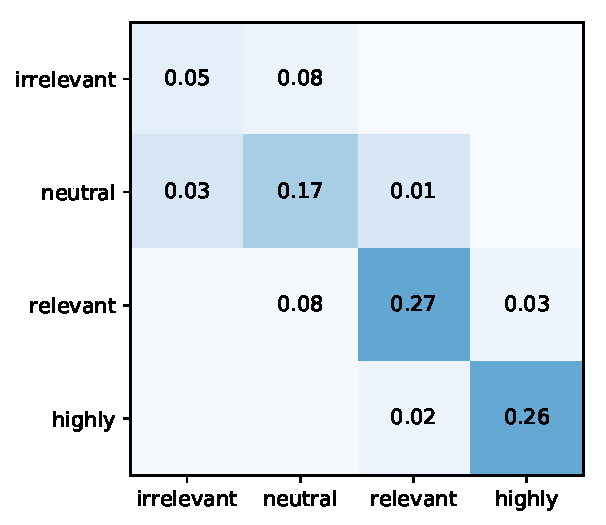
\includegraphics[width=\linewidth]{conf_full}
%		\caption{Trained on all samples}
%	\end{subfigure}%
%	~ 
%	\begin{subfigure}[t]{0.5\linewidth}
%		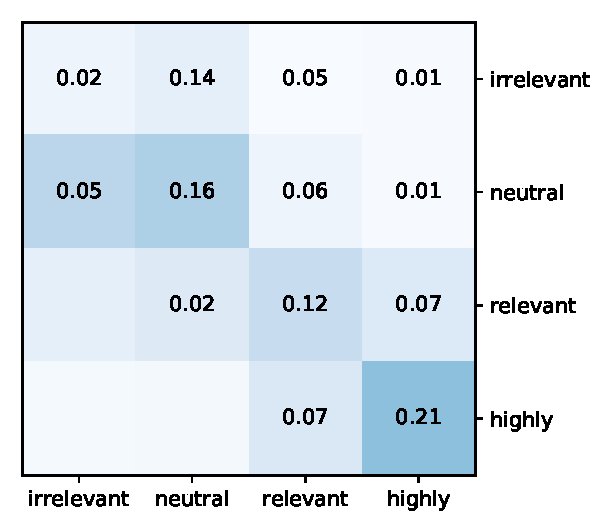
\includegraphics[width=\linewidth]{conf_role}
%		\caption{Trained on role samples}
%	\end{subfigure}
%	\caption{Normalised aggregated confusion matrices for the model with different training sets}
%	\label{fig:confmatrix}
%\end{figure}
%


%\begin{table}
%	\caption{Experimental results for bag-of-words (BOW), embedding (EMB), syntax (SYN) features}, and ensemble (ENS)
%	\label{tab:results}
%	\begin{tabular}{lcc}
%		\toprule
%		Approach & NDCG & $\sigma ($NDCG$)$\\
%		\midrule
%		Baseline (random) & 0.87 & 0.07\\
%		Baseline (worst) & 0.73 & 0.13\\
%		\midrule
%		%F1 full 0.73 std=0.27
%		%F1 role 0.49 std=0.17
%		BOW, full set, categorical & 0.97 & 0.04 \\
%		BOW, role based, categorical & 0.92 & 0.07  \\
%		BOW, full set, continuous & \textbf{0.98} & 0.03 \\
%		BOW, role based, continuous & 0.93 & 0.07 \\
%		\midrule
%		% F1 full 0.41 std=0.16
%		% F1 role 0.38 std=0.21
%		EMB, full set, categorical & 0.91 & 0.07 \\
%		EMB, role based, categorical & 0.89 & 0.07  \\
%		EMB, full set, continuous & 0.92 & 0.07 \\
%		EMB, role based, continuous & 0.90 & 0.08 \\
%		\midrule
%		% F1 full 0.43 std=0.26
%		% F1 role 0.39 std=0.26
%		SYN, full set, categorical & 0.93 & 0.07 \\
%		SYN, role based, categorical & 0.92 & 0.07  \\
%		SYN, full set, continuous & 0.94 & 0.06 \\
%		SYN, role based, continuous & 0.92 & 0.08 \\
%		\midrule
%		% F1 full 0.46 std=0.22
%		% F1 role 0.39 std=0.20
%		ENS, full set, categorical & 0.93 & 0.06 \\
%		ENS, role based, categorical & 0.91 & 0.07  \\
%		ENS, full set, continuous & 0.93 & 0.06 \\
%		ENS, role based, continuous & 0.92 & 0.07 \\
%		\bottomrule
%	\end{tabular}
%\end{table}
